\documentclass[11pt,a4paper,fleqn]{article}
\usepackage[margin=1in]{geometry}
\usepackage{graphicx} 
\usepackage{pdfpages}
\begin{document}
\begin{center}
\textbf{CS6140 Machine Learning Fall 2014 Homework 3, Wei Luo }\\
\end{center}
\textbf{PROBLEM 1}\\
\\
Using Gaussian Discriminant Analysis, I got:  \\
average train error rate: 0.091212
average test error rate: 0.096498 \\
Since the average accuracy is over 0.9, it seems to me that the gaussian assumption holds for this data set.\\
\\
\textbf{PROBLEM 2}\\
\\
The Error Table for Na\"{i}ve Bayes Classifier, Model with Bernoulli Random Variables:\\
\begin{tabular}{|c|c|c|c|}
\hline
fold\#&false positive rate&false negative rate&overall error rate\\
\hline
1&0.142322&0.067010&0.110629\\
\hline
2&0.134021&0.112426&0.126087\\
\hline
3&0.123288&0.089286&0.110870\\
\hline
4&0.104651&0.084158&0.095652\\
\hline
5&0.119718&0.062500&0.097826\\
\hline
6&0.127208&0.056497&0.100000\\
\hline
7&0.118467&0.127168&0.121739\\
\hline
8&0.114695&0.049724&0.089130\\
\hline
9&0.128571&0.083333&0.110870\\
\hline
10&0.123596&0.062176&0.097826\\
\hline
average&0.12365375&0.07942785&0.10606291\\
\hline
\end{tabular}\\
\\
The Error Table for Na\"{i}ve Bayes Classifier, Model with Gaussian Random Variables:\\
\begin{tabular}{|c|c|c|c|}
\hline
fold\#&false positive rate&false negative rate&overall error rate\\
\hline
1&0.186207&0.140351&0.169197\\
\hline
2&0.121622&0.091463&0.110870\\
\hline
3&0.102273&0.056122&0.082609\\
\hline
4&0.138996&0.084577&0.115217\\
\hline
5&0.175000&0.077778&0.136957\\
\hline
6&0.178832&0.112903&0.152174\\
\hline
7&0.136842&0.085714&0.117391\\
\hline
8&0.138686&0.096774&0.121739\\
\hline
9&0.199301&0.137931&0.176087\\
\hline
10&0.157143&0.094444&0.132609\\
\hline
average&0.15349013&0.09780588&0.13148496\\
\hline
\end{tabular}\\
\\
The Error Table for Na\"{i}ve Bayes Classifier (4-bins Histogram):\\
\begin{tabular}{|c|c|c|c|}
\hline
fold\#&false positive rate&false negative rate&overall error rate\\
\hline
1&0.086957&0.221622&0.140998\\
\hline
2&0.097222&0.151163&0.117391\\
\hline
3&0.076642&0.139785&0.102174\\
\hline
4&0.103321&0.190476&0.139130\\
\hline
5&0.064982&0.218579&0.126087\\
\hline
6&0.084559&0.196809&0.130435\\
\hline
7&0.078292&0.195531&0.123913\\
\hline
8&0.081851&0.201117&0.128261\\
\hline
9&0.094737&0.194286&0.132609\\
\hline
10&0.063604&0.225989&0.126087\\
\hline
average&0.08321663&0.19353558&0.12670848\\
\hline
\end{tabular}\\
\\
The Error Table for Na\"{i}ve Bayes Classifier (9-bins Histogram):\\
\begin{tabular}{|c|c|c|c|}
\hline
fold\#&false positive rate&false negative rate&overall error rate\\
\hline
1&0.032374&0.251366&0.119306\\
\hline
2&0.025180&0.340659&0.150000\\
\hline
3&0.025271&0.371585&0.163043\\
\hline
4&0.007692&0.485000&0.215217\\
\hline
5&0.021818&0.356757&0.156522\\
\hline
6&0.027119&0.400000&0.160870\\
\hline
7&0.027027&0.358209&0.171739\\
\hline
8&0.049123&0.291429&0.141304\\
\hline
9&0.023649&0.329268&0.132609\\
\hline
10&0.017544&0.365714&0.150000\\
\hline
average&0.02567962&0.3549987&0.15606102\\
\hline
\end{tabular}\\
\\
The ROC curves and AUC for each classifier is:\\
\includegraphics[scale=0.75]{ROC_Naive_Bayes.png}\\
\\ \\ \\ \\ \\ \\ \\ \\
\textbf{PROBLEM 3}\\
(next page)
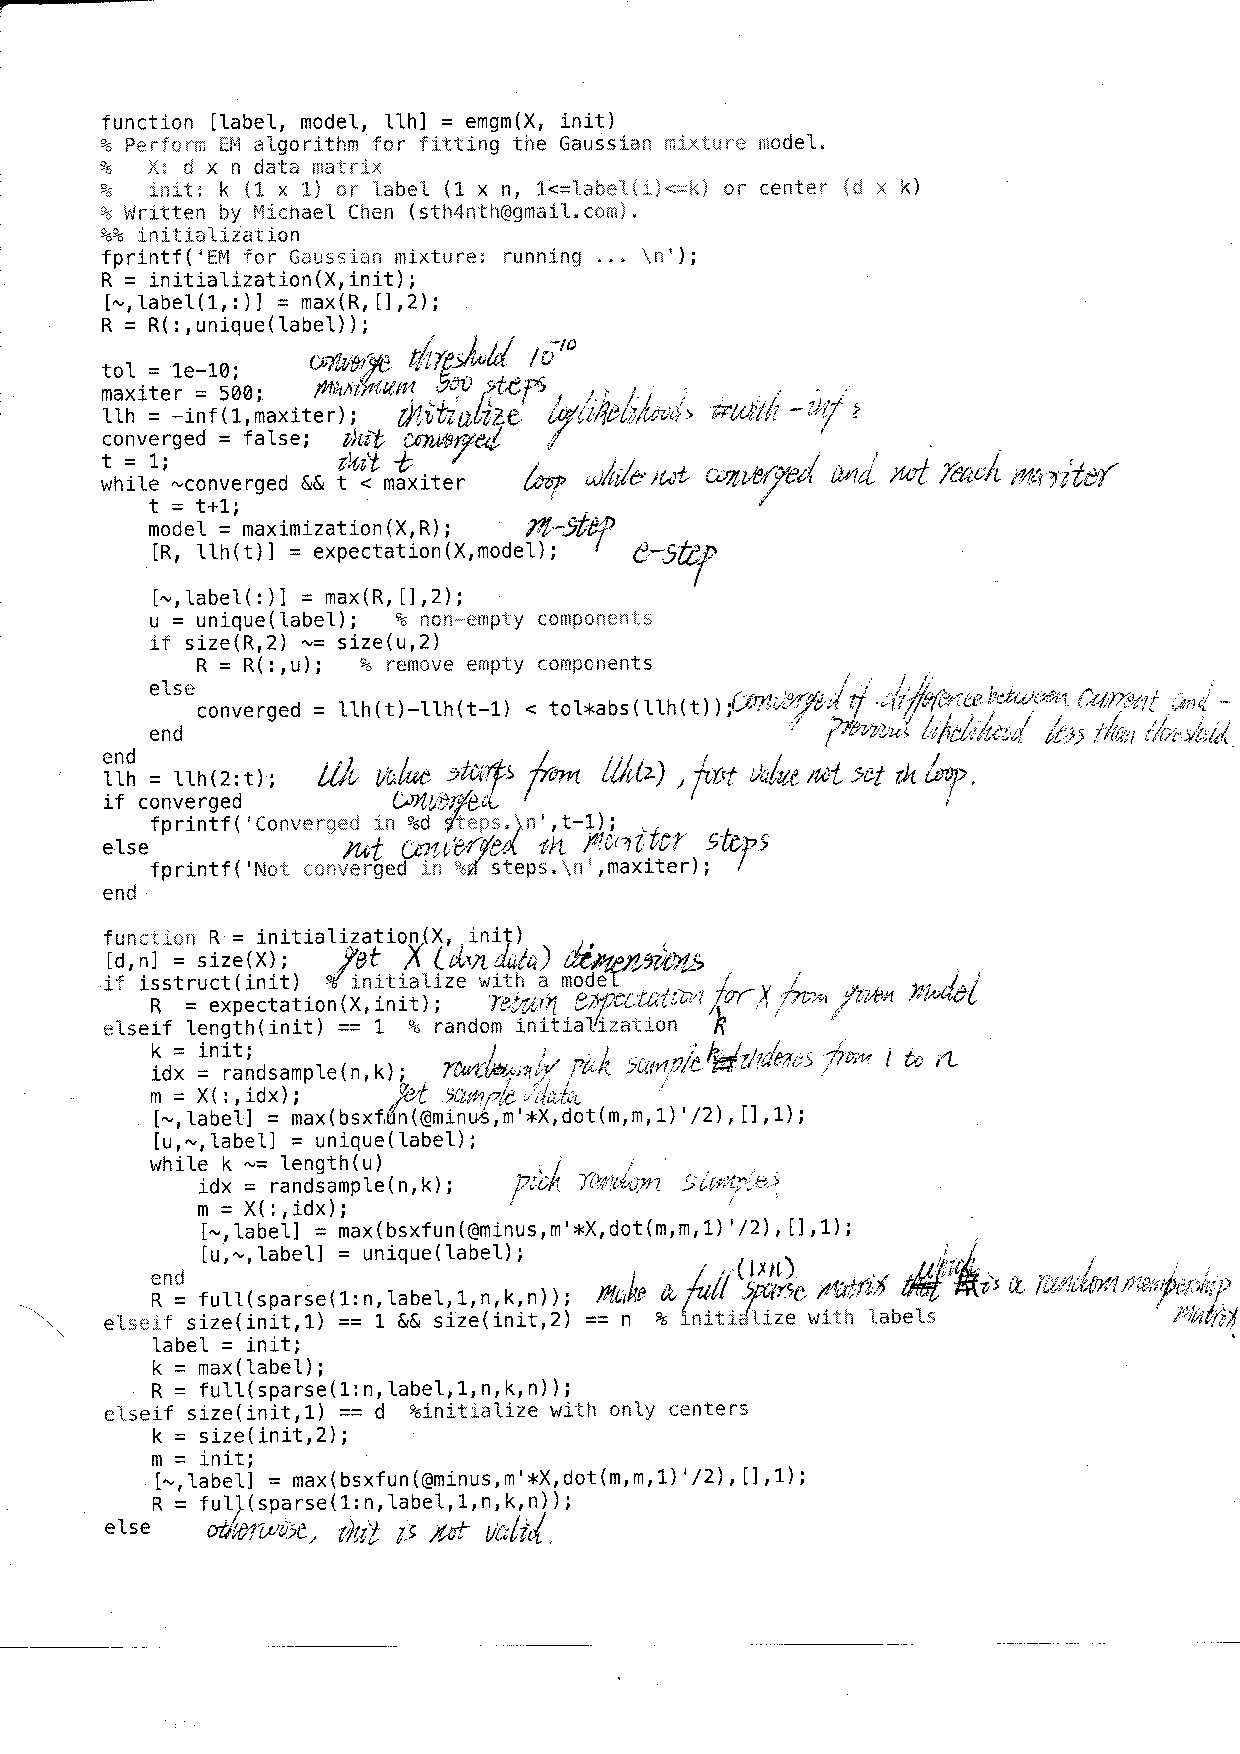
\includepdf[pages={1,2}]{102-scan.pdf}
\newpage \noindent 
\textbf{PROBLEM 4}\\
\textbf{A)} The results for 2 gaussian:\\
\indent $\mathbf{Gaussian_1}$: points: 1981; mean: [2.94846981, 3.0421113]\\
\indent covariance: [[0.8992528, 0.01219505], [0.01219505, 2.96950283]] \\
\indent $\mathbf{Gaussian_2}$: points: 4019; mean: [7.0078808, 3.98162176]\\
\indent covariance: [[0.95936573, 0.4865028], [0.4865028, 0.99568567]] \\
\textbf{B)} The results for 3 gaussian:\\
\indent $\mathbf{Gaussian_1}$: points: 3098; mean: [6.98857865, 4.03307065]\\
\indent covariance: [[1.00480526, 0.49076192], [0.49076192, 1.0080817]] \\
\indent $\mathbf{Gaussian_2}$: points: 1945; mean: [2.91656552, 2.8932281]\\
\indent covariance: [[0.86404608, -0.20507606], [-0.20507606, 2.9738529]] \\
\indent $\mathbf{Gaussian_3}$: points: 4957; mean: [4.99043274, 7.03134783]\\
\indent covariance: [[0.91578388, 0.18253052], [0.18253052, 0.90038684]] \\
\\
\\
\textbf{PROBLEM 5}\\
\textbf{a)}
$$\frac{P(B|A,C)P(A|C)}{P(B|C)}=\frac{P(A,B,C)/P(A,C)*P(A,C)/P(C)}{P(B,C)/P(C)}=\frac{P(A,B,C)}{P(B,C)}=P(A|B,C)$$
\textbf{b)}
The prior probability of the coin being fair is $P(F)=\frac{F}{F+1}$. So the prior probability of the coin being double-headed is $P(D) = 1 - P(F) = \frac{1}{F+1}$. If we see $n$ heads in a row, the probability that the coon is fair is: $P(F|nH) = \frac{P(nH|F)P(F)}{P(nH)}$;  the probability that the coon is fair is: $P(D|nH) = \frac{P(nH|D)P(D)}{P(nH)}$. If the coin is fair, the probability of seeing a head is $P(H|F) = \frac{1}{2}$. the probability of seeing $n$ heads in a row is $P(nH|F) = P(H|F)^n = (\frac{1}{2})^n$. If the coin is double-headed, the probability of seeing a head and $n$ head in a row is $P(H|D)=P(nH|D)=1$. We want a better than even chance that the coin is double-headed, which means $P(D|nH)>P(F|nH)$. So $\frac{P(nH|D)P(D)}{P(nH)}>\frac{P(nH|F)P(F)}{P(nH)}$. So $1*\frac{1}{F+1}>(\frac{1}{2})^n*\frac{F}{F+1}$.\\
We get $n > \log_2F$. So we need to see more than  $\log_2F$ heads in a row to become convinced that there is a better than even chance that the coin is double-headed.\\
\\
\\
\textbf{PROBLEM 6}\\
Flip different number of coins with different probabilities. Then run em algorithm:\\ \\
\begin{tabular}{|c|ll|}
\hline
$\pi$&0.8&0.2\\
$em\_\pi$&0.84163594&0.15836406\\
\hline
probs&0.75&0.4\\
em\_probs&0.74193735&0.386823\\
\hline
\end{tabular}\\ \\ \\
\begin{tabular}{|c|ll|}
\hline
$\pi$&0.4&0.6\\
$em\_\pi$&0.41665103&0.58334897\\
\hline
probs&0.9&0.2\\
em\_probs&0.89850985&0.19634036\\
\hline
\end{tabular}\\ \\ \\
\begin{tabular}{|c|ll|}
\hline
$\pi$&0.1&0.9\\
$em\_\pi$&0.29550855&0.70449145\\
\hline
probs&0.45&0.51\\
em\_probs&0.45889733&0.51653134\\
\hline
\end{tabular}\\
\begin{tabular}{|c|lll|}
\hline
$\pi$&0.2&0.3&0.5\\
$em\_\pi$&0.19472662&0.31741561&0.48785777\\
\hline
probs&0.99&0.47&0.08\\
em\_probs&0.99373054&0.48164992&0.07176479\\
\hline
\end{tabular}\\ \\ \\
\begin{tabular}{|c|lllll|}
\hline
$\pi$&0.1&0.1&0.2&0.3&0.3\\
$em\_\pi$&0.13627108&0.0884572&0.11475013&0.3240638&0.33645778\\
\hline
probs&0.98&0.69&0.38&0.21&0.03\\
em\_probs&0.97007034&0.64665238&0.30068529&0.28223276&0.03697732\\
\hline
\end{tabular}\\ \\ \\
\\
\textbf{PROBLEM 7}\\
Tried with K = \{1,2,4,9\}. The average error rates are as follows:\\
\begin{tabular}{|c|c|c|c|c|}
\hline
K&1&2&4&9\\
\hline
Error Rate&0.132321&0.130152&0.097614&0.091106\\
\hline
\end{tabular}\\ \\
And the ROC curve for each K is:\\
\includegraphics[scale=0.75]{ROC_Gaussian_Mixtures.png}\\
\end{document}